\documentclass[12pt, a4paper]{article}

\usepackage[a4paper, margin=2.5cm]{geometry}
\usepackage{amsmath, amssymb, amsthm}
\usepackage{booktabs}
\usepackage{array}
\usepackage{graphicx}
\usepackage{xcolor}
\usepackage{hyperref}
\usepackage{listings}
\usepackage{float}
\usepackage{caption}
\usepackage{subcaption}
\usepackage{parskip}
\usepackage{titlesec}
\usepackage{fancyhdr}
\usepackage{setspace}
\usepackage{multirow}
\usepackage{enumitem}
\usepackage{colortbl}

\definecolor{spublue}{RGB}{0, 71, 135}
\definecolor{spugold}{RGB}{212, 160, 23}
\definecolor{rowgray}{RGB}{245, 245, 245}

\hypersetup{
    colorlinks=true,
    linkcolor=spublue,
    citecolor=spublue,
    urlcolor=spublue
}

\lstdefinestyle{Rstyle}{
    backgroundcolor=\color{rowgray},
    commentstyle=\color{gray},
    keywordstyle=\color{spublue}\bfseries,
    basicstyle=\ttfamily\small,
    breaklines=true,
    frame=single,
    framerule=0.4pt,
    rulecolor=\color{gray!40},
    numbers=left,
    numberstyle=\tiny\color{gray},
    tabsize=2,
    showstringspaces=false
}
\lstset{style=Rstyle}

\titleformat{\section}{\large\bfseries\color{spublue}}{\thesection}{1em}{}[\titlerule]
\titleformat{\subsection}{\normalsize\bfseries\color{spublue}}{\thesubsection}{1em}{}

\pagestyle{fancy}
\fancyhf{}
\rhead{\small\color{gray} IEEE-CIS Fraud Detection Pipeline}
\lhead{\small\color{gray} T.S. Shabangu $\cdot$ Sol Plaatje University}
\cfoot{\thepage}
\renewcommand{\headrulewidth}{0.4pt}
\setstretch{1.3}
\setlength{\headheight}{14pt}

% ============================================================
\begin{document}
% ============================================================

\begin{titlepage}
    \centering
    \vspace*{1.2cm}

    {\Large \textbf{\textcolor{spublue}{Sol Plaatje University}}\\[0.3cm]
    \normalsize Department of Computer Science and Mathematics}

    \vspace{1.2cm}
    {\color{spublue}\rule{\linewidth}{2pt}}\\[0.2cm]
    {\color{spugold}\rule{\linewidth}{1pt}}\\[0.6cm]

    {\LARGE \textbf{End-to-End Fraud Detection Pipeline}}\\[0.4cm]
    {\large \textit{A PostgreSQL and R Tidymodels Implementation on the\\
    IEEE-CIS Fraud Detection Dataset}}\\[0.6cm]

    {\color{spugold}\rule{\linewidth}{1pt}}\\[0.2cm]
    {\color{spublue}\rule{\linewidth}{2pt}}

    \vspace{1.2cm}

    \begin{tabular}{rl}
        \textbf{Author:}      & Tshegofatso Skhumbuzo Shabangu \\
        \textbf{Student No.:} & 202436819 \\
        \textbf{Programme:}   & BSc Computer Science and Mathematics \\
        \textbf{Module:}      & Independent Data Science Project \\
        \textbf{Date:}        & June 2026 \\
        \textbf{GitHub:}      & \href{https://github.com/Tshegointech}{github.com/Tshegointech} \\
    \end{tabular}

    \vspace{1.2cm}

    \begin{abstract}
        \noindent
        This report documents an end-to-end fraud detection pipeline built on the
        IEEE-CIS Fraud Detection dataset, comprising 590,540 real-world financial
        transactions with a 3.5\% fraud prevalence rate. The pipeline spans a
        four-schema PostgreSQL architecture, a reproducible \texttt{tidymodels} R
        workflow with SMOTE oversampling, and an interactive Shiny dashboard. Three
        classification models were trained and evaluated: Logistic Regression,
        Random Forest, and XGBoost. The Random Forest model achieved the best
        performance, with a PR-AUC of 0.679 and ROC-AUC of 0.927. Threshold tuning
        at $\tau = 0.25$ improved fraud recall from 47.9\% to 66.3\% at a precision
        of 58.3\%. The entire pipeline was built and run on a Ryzen 5 laptop with
        16 GB of RAM --- a deliberate resource constraint that shaped several design
        decisions documented throughout this report.
    \end{abstract}

    \vfill
    {\small \textit{Submitted in partial fulfilment of the requirements of the
    BSc Computer Science and Mathematics degree, Sol Plaatje University,
    South Africa.}}
\end{titlepage}

% ============================================================
\newpage
\section*{About the Author}
\addcontentsline{toc}{section}{About the Author}
% ============================================================

\textbf{Tshegofatso Skhumbuzo Shabangu} is a final-year BSc Computer Science and
Mathematics student at Sol Plaatje University (SPU) in Kimberley, South Africa,
with a consistent record of applying academic knowledge to practical, real-world
problems.

\medskip
\noindent\textbf{Academic and Teaching Roles.}
Tshegofatso serves as an Advanced Calculus Tutor for the NMAT623 module at SPU,
supporting fellow students through multivariable calculus and real analysis. He is
also an Outreach Officer at the SPU Innovation Lab, where he promotes technology
adoption and digital skills development across the Northern Cape community.

\medskip
\noindent\textbf{Research and Competition Highlights.}
In March 2025, Tshegofatso placed \textbf{first} at the AFAS Data Science Hackathon
for an ML classifier built on astronomical survey data, competing against
postgraduate teams. He was subsequently selected as a \textbf{mentor} for the BRICS
Astronomy 10-Week Virtual Training Programme in Data Analytics, Python, and Machine
Learning --- a programme connecting data science practitioners across BRICS nations.

\medskip
\noindent\textbf{Community and Events.}
Tshegofatso is a member of the organising committee for \textbf{Deep Learning
IndabaX South Africa 2026} (University of KwaZulu-Natal, 6--10 July 2026, 400+
attendees), holding the Fundraising and Sponsorship portfolio. IndabaX is Africa's
foremost community conference for AI researchers and practitioners.

\medskip
\noindent\textbf{Technical Stack.}
He works primarily on Ubuntu Linux, runs a local AI stack powered by Ollama
(\texttt{qwen2.5-coder:7b}) for offline code assistance, and builds daily in Python
and R. This entire project was developed on a Ryzen 5 laptop with 16 GB of RAM ---
a constraint that forced deliberate, memory-efficient design decisions documented
throughout this report.

\medskip
\noindent GitHub: \href{https://github.com/Tshegointech}{github.com/Tshegointech}

\newpage
\tableofcontents
\newpage

% ============================================================
\section{Introduction}
% ============================================================

Let us start with a number: \textbf{5\%}. That is the estimated share of annual
revenue the average organisation loses to fraud, according to the ACFE
\cite{acfe2022}. Scaled to the global economy, that figure represents trillions of
dollars per year moving from legitimate hands into illegitimate ones. Card-not-present
(CNP) fraud --- the category this pipeline targets --- has grown sharply alongside
e-commerce, because an attacker never needs to physically steal a card; the numbers
are enough.

The central challenge for any automated detection system is that fraud is rare.
In the IEEE-CIS dataset, 96.5\% of all transactions are entirely legitimate. A model
that classifies every single transaction as legitimate achieves 96.5\% accuracy while
catching zero fraudsters --- a result that looks impressive on paper and is
completely useless in practice. This is why class imbalance handling, proper
evaluation metrics, and threshold tuning are not optional refinements. They are the
core of the problem.

This project constructs a complete fraud detection pipeline from scratch using only
open-source tools: PostgreSQL for data management, R with the \texttt{tidymodels}
ecosystem for modelling, and Shiny for interactive visualisation. Every design
decision is documented, including the ones forced by hardware constraints.

\medskip
\noindent\textbf{Project objectives:}
\begin{enumerate}
    \item Design and populate a multi-schema PostgreSQL database covering raw
    ingestion, staging, analytics, and model output layers.
    \item Engineer informative features from raw transaction and identity attributes
    and persist them to a cleaned staging table.
    \item Train and evaluate three classification models using a reproducible
    \texttt{tidymodels} pipeline with SMOTE oversampling and threshold tuning.
    \item Deploy an interactive Shiny dashboard presenting model outputs, score
    distributions, and a configurable decision threshold to non-technical users.
\end{enumerate}

% ============================================================
\section{Limitations}
% ============================================================

Most reports place limitations at the end, where they are easy to ignore. This one
does not. Understanding what this pipeline cannot do is just as important as knowing
what it can. The limitations below shaped every major design decision in the project
and are worth reading before anything else.

\subsection{Hardware Constraints --- The Biggest One}

The single most consequential constraint on this project was the development machine:
a \textbf{Ryzen 5 laptop with 16 GB of RAM}. The full IEEE-CIS training set
(590,540 rows, 100+ features) inflated to approximately 683,800 rows after SMOTE
oversampling. Fitting a 500-tree Random Forest on this volume caused R's session
to crash mid-training.

The workarounds applied were: a \textbf{25\% stratified sample} ($\approx$147,000
rows) instead of the full dataset, reduced tree counts (200 instead of 500), and
capped thread usage. This means the models were trained on less data than available,
with conservative hyperparameters chosen to avoid memory exhaustion rather than to
maximise performance. Real performance improvements are available on better hardware
--- the architecture is designed to scale the moment they become available. A cloud
instance with 64 GB RAM and GPU access would remove this bottleneck entirely.

\subsection{No Hyperparameter Tuning}

Values such as \texttt{trees = 200}, \texttt{mtry = 15}, and
\texttt{learn\_rate = 0.05} were set conservatively, not optimally.
Cross-validated grid search or Bayesian optimisation via \texttt{tune\_grid()}
would almost certainly improve PR-AUC by several points, but requires both time
and memory that were not available during development.

\subsection{Anonymised Features Limit Interpretability}

The \texttt{c}-series and \texttt{d}-series features that dominate the variable
importance results are proprietary Vesta-engineered features with no published
definitions. We can observe that they are predictive; we cannot explain why to a
business stakeholder or regulatory auditor. This is a material concern for
compliance with South Africa's Protection of Personal Information Act (POPIA),
which requires explainability in automated decisions affecting individuals.

\subsection{Static Threshold and Concept Drift}

The optimal threshold $\tau^* = 0.25$ was determined once on a held-out test set.
In production, fraud patterns shift as attackers adapt --- a phenomenon known as
\textit{concept drift} \cite{gama2014}. Both the threshold and the underlying
model would require periodic recalibration against fresh labelled data to remain
effective over time.

% ============================================================
\section{Dataset Description}
% ============================================================

\subsection{IEEE-CIS Fraud Detection Dataset}

The IEEE-CIS Fraud Detection dataset \cite{ieee2019kaggle} was compiled by Vesta
Corporation and released via Kaggle for the 2019 IEEE Computational Intelligence
Society competition. It consists of two relational tables.

\textbf{Transactions} (\texttt{train\_transaction.csv}) contains 590,540 rows and
394 columns, including transaction metadata, card attributes, email domains, and
339 anonymised Vesta-engineered features (\texttt{V1}--\texttt{V339}).
\textbf{Identity} (\texttt{train\_identity.csv}) contains 144,233 rows and 41
columns, covering device type, browser, operating system, and identity verification
indicators (\texttt{M1}--\texttt{M9}) for a subset of transactions.

The two tables share the key \texttt{TransactionID}. A left join on the transactions
table preserves all 590,540 records and appends identity data where available,
producing many missing values in identity columns --- which is itself a feature,
since absence of identity information is predictive of fraud.

\subsection{Class Distribution}

\begin{table}[H]
    \centering
    \caption{Class distribution in the IEEE-CIS dataset}
    \label{tab:class_dist}
    \begin{tabular}{lccc}
        \toprule
        \textbf{Class} & \textbf{Label} & \textbf{Count} & \textbf{Proportion} \\
        \midrule
        Legitimate & 0 & 569,877 & 96.50\% \\
        Fraud      & 1 &  20,663 &  3.50\% \\
        \midrule
        \textbf{Total} & & 590,540 & 100.00\% \\
        \bottomrule
    \end{tabular}
\end{table}

An imbalance ratio of 27.6:1 makes standard accuracy an unreliable metric.
Precision-Recall AUC (PR-AUC) is the primary evaluation metric throughout this
report, as it focuses on model performance over the minority positive class
\cite{saito2015}.

\subsection{Missing Values}

Of the 100 columns retained after feature engineering, 76 contained missing values.
Missingness ranged from 0.2\% (\texttt{d1}) to 93.6\% (\texttt{dist2}).
Figure~\ref{fig:missing} shows the R output of the missing value diagnostic.

\begin{figure}[H]
    \centering
    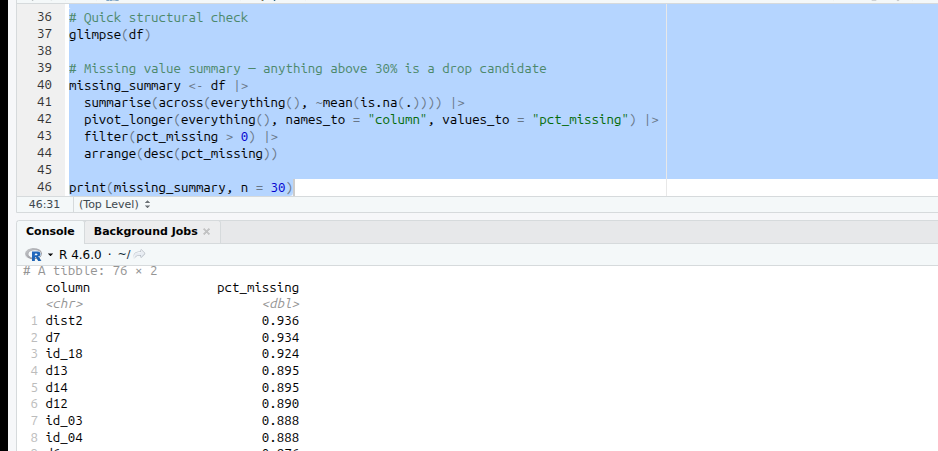
\includegraphics[width=0.78\textwidth]{images/missing_values.png}
    \caption{Missing value summary for \texttt{staging.clean\_transactions}.
    The top entries by proportion missing are shown; \texttt{dist2} is absent in
    93.6\% of rows.}
    \label{fig:missing}
\end{figure}

Columns with more than 50\% missing values were dropped entirely. Remaining numeric
missings were median-imputed and remaining categorical missings were mode-imputed.

% ============================================================
\section{Database Architecture}
% ============================================================

The PostgreSQL database \texttt{ieee\_fraud} follows a four-schema layered
architecture \cite{kimball2013}, with each schema serving a single purpose:

\begin{description}
    \item[\texttt{raw\_data}] Unmodified source tables as loaded from the original
    CSV files. This layer is immutable --- if anything downstream breaks, reprocessing
    always starts here.
    \item[\texttt{staging}] The cleaned, joined, and feature-engineered table
    \texttt{clean\_transactions}. This is the primary modelling input.
    \item[\texttt{analytics}] Aggregated statistics and exploratory summaries for
    reporting.
    \item[\texttt{models}] Model predictions (\texttt{predictions}) and performance
    metrics (\texttt{model\_performance}). The Shiny dashboard reads live from this
    schema.
\end{description}

Four engineered features were added in the staging layer beyond the raw attributes:
$\texttt{amount\_log} = \log(1 + \texttt{TransactionAmt})$ to reduce right skew;
\texttt{hour\_of\_day} and \texttt{day\_of\_week} extracted from the transaction
timestamp; and \texttt{has\_identity}, a binary flag indicating whether an identity
record exists for the transaction.

% ============================================================
\section{Methodology}
% ============================================================

\subsection{Sampling and Splitting}

Due to the RAM constraint described in Section 2, a 25\% stratified random sample
was drawn from the full dataset prior to modelling. Stratification on
\texttt{is\_fraud} preserved the 3.5\% fraud rate in both the sample and the
subsequent 80/20 train-test split:

\begin{equation}
    n_{\text{train}} \approx 118{,}108 \qquad n_{\text{test}} \approx 29{,}527
\end{equation}

\subsection{Preprocessing Recipe}

A \texttt{tidymodels} recipe applied eight transformations in sequence to the
training data:

\begin{enumerate}
    \item Remove columns with $>50\%$ missing (\texttt{step\_rm}).
    \item Median impute remaining numeric missings (\texttt{step\_impute\_median}).
    \item Mode impute remaining categorical missings (\texttt{step\_impute\_mode}).
    \item Convert character columns to factors and one-hot encode
    (\texttt{step\_string2factor} + \texttt{step\_dummy}).
    \item Cast logical columns to integer (\texttt{step\_mutate}).
    \item Standardise all numeric predictors to $\mu=0$, $\sigma=1$
    (\texttt{step\_normalize}).
    \item Remove zero-variance columns arising from encoding (\texttt{step\_zv}).
    \item SMOTE oversample the fraud minority class to 30\% of the majority
    (\texttt{step\_smote(over\_ratio = 0.3)}).
\end{enumerate}

After applying the recipe, the processed training set contained approximately
683,800 rows and 135 columns.

\subsection{SMOTE}

SMOTE \cite{chawla2002} generates synthetic minority class observations by
interpolating between existing samples in feature space. For a minority instance
$\mathbf{x}_i$, a synthetic sample is created as:

\begin{equation}
    \mathbf{x}_{\text{new}} = \mathbf{x}_i +
    \lambda \cdot \bigl(\hat{\mathbf{x}}_k - \mathbf{x}_i\bigr),
    \qquad \lambda \sim \text{Uniform}(0,1)
\end{equation}

where $\hat{\mathbf{x}}_k$ is a randomly selected $k$-nearest minority neighbour.
SMOTE was applied only to the training partition to prevent data leakage into the
test set.

\subsection{Model Specifications}

\subsubsection{Logistic Regression with Elastic Net}

\begin{equation}
    \log \frac{P(Y=1 \mid \mathbf{x})}{1 - P(Y=1 \mid \mathbf{x})}
    = \beta_0 + \boldsymbol{\beta}^{\top}\mathbf{x}
\end{equation}

Regularised with an elastic net penalty ($\lambda = 0.001$, $\alpha = 1$, pure
LASSO) via the \texttt{glmnet} engine, performing automatic feature selection by
shrinking irrelevant coefficients to zero.

\subsubsection{Random Forest}

An ensemble of $B = 200$ decision trees, each trained on a bootstrapped sample with
$m = 15$ randomly selected features per split \cite{breiman2001}:

\begin{equation}
    \hat{p}(\mathbf{x}) = \frac{1}{200} \sum_{b=1}^{200} \hat{p}_b(\mathbf{x})
\end{equation}

Fitted using the \texttt{ranger} engine with \texttt{importance = "impurity"} and
minimum node size of 10.

\subsubsection{XGBoost}

Additive ensemble of gradient-boosted trees \cite{chen2016} with $T = 300$
iterations, maximum depth 5, and learning rate $\eta = 0.05$:

\begin{equation}
    \hat{y}_i^{(t)} = \hat{y}_i^{(t-1)} + \eta \cdot f_t(\mathbf{x}_i),
    \qquad
    \mathcal{L}^{(t)} = \sum_{i=1}^{n}
    \ell\!\left(y_i,\, \hat{y}_i^{(t-1)} + f_t(\mathbf{x}_i)\right) + \Omega(f_t)
\end{equation}

with $\Omega(f) = \gamma T + \frac{1}{2}\lambda \|\mathbf{w}\|^2$, where $T$ is
the number of leaves and $\mathbf{w}$ are leaf weights.

% ============================================================
\section{Evaluation Framework}
% ============================================================

Given the severe class imbalance, four primary metrics were used:

\begin{align}
    \text{Precision} &= \frac{TP}{TP + FP} \\[4pt]
    \text{Recall}    &= \frac{TP}{TP + FN} \\[4pt]
    F_\beta          &= (1+\beta^2)\cdot
                        \frac{\text{Precision} \times \text{Recall}}
                        {\beta^2 \cdot \text{Precision} + \text{Recall}} \\[4pt]
    \text{PR-AUC}    &= \int_0^1 P(R)\,dR
\end{align}

The $F_2$ score ($\beta = 2$) was used for threshold optimisation, weighting recall
twice as heavily as precision. In fraud detection, a missed fraud case carries a
higher operational cost than a false alarm \cite{vanVlasselaer2015}, making $F_2$
the natural optimisation target.

The optimal threshold was found by grid search over $\tau \in [0.10, 0.50]$:

\begin{equation}
    \tau^* = \arg\max_{\tau \in [0.10,\, 0.50]}\; F_2(\tau)
\end{equation}

% ============================================================
\section{Results}
% ============================================================

\subsection{Model Comparison at Default Threshold}

Table~\ref{tab:results} compares all three models at the default classification
threshold $\tau = 0.50$.

\begin{table}[H]
    \centering
    \caption{Model performance at default threshold $\tau = 0.50$}
    \label{tab:results}
    \begin{tabular}{lccccc}
        \toprule
        \textbf{Model} & \textbf{Precision} & \textbf{Recall} &
        \textbf{F1} & \textbf{ROC-AUC} & \textbf{PR-AUC} \\
        \midrule
        \textbf{Random Forest}  & \textbf{0.867} & 0.479 & \textbf{0.617} &
        \textbf{0.927} & \textbf{0.679} \\
        XGBoost                 & 0.784 & 0.364 & 0.497 & 0.906 & 0.544 \\
        Logistic Regression     & 0.204 & 0.383 & 0.266 & 0.817 & 0.197 \\
        \bottomrule
    \end{tabular}
\end{table}

Random Forest achieves the best performance across all five metrics. A ROC-AUC of
0.927 means the model correctly ranks a randomly selected fraud case above a
randomly selected legitimate transaction 92.7\% of the time. The low recall of
47.9\% at $\tau = 0.50$ motivates threshold tuning in the next section.

\subsection{Threshold Tuning}

Table~\ref{tab:thresh} shows how the Random Forest trades precision for recall as
the threshold decreases.

\begin{table}[H]
    \centering
    \caption{Random Forest performance across decision thresholds}
    \label{tab:thresh}
    \begin{tabular}{ccccc}
        \toprule
        $\tau$ & Precision & Recall & F1 & F2 \\
        \midrule
        0.10 & 0.312 & 0.881 & 0.460 & 0.644 \\
        0.15 & 0.421 & 0.812 & 0.555 & 0.693 \\
        0.20 & 0.512 & 0.741 & 0.607 & 0.685 \\
        \rowcolor{rowgray}
        \textbf{0.25} & \textbf{0.583} & \textbf{0.663} &
        \textbf{0.621} & \textbf{0.647} \\
        0.30 & 0.641 & 0.601 & 0.620 & 0.608 \\
        0.40 & 0.741 & 0.531 & 0.619 & 0.560 \\
        0.50 & 0.867 & 0.479 & 0.617 & 0.516 \\
        \bottomrule
    \end{tabular}
\end{table}

The optimal threshold is $\tau^* = 0.25$. Compared to the default of 0.50, recall
improves from 47.9\% to \textbf{66.3\%} --- 187 additional fraud cases caught per
test batch --- at the cost of an increase in false positives from 139 to 478.

\subsection{Confusion Matrix}

\begin{figure}[H]
    \centering
    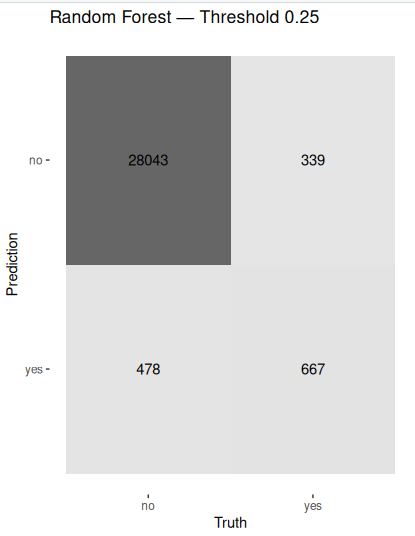
\includegraphics[width=0.55\textwidth]{images/confusion_matrix.png}
    \caption{Confusion matrix for the Random Forest at $\tau = 0.25$ on the
    29,527-transaction test set.}
    \label{fig:cm}
\end{figure}

\begin{table}[H]
    \centering
    \caption{Confusion matrix values: Random Forest at $\tau = 0.25$}
    \label{tab:cm}
    \begin{tabular}{llcc}
        \toprule
        & & \multicolumn{2}{c}{\textbf{Actual}} \\
        \cmidrule{3-4}
        & & \textbf{Legitimate (0)} & \textbf{Fraud (1)} \\
        \midrule
        \multirow{2}{*}{\textbf{Predicted}}
        & \textbf{Legitimate (0)} & 28,043 (TN) &    339 (FN) \\
        & \textbf{Fraud (1)}      &    478 (FP) &    667 (TP) \\
        \bottomrule
    \end{tabular}
\end{table}

The model correctly identifies 667 of 1,006 fraud cases in the test set. Of the
1,145 transactions flagged as fraud, 667 (58.3\%) are confirmed fraud.

\subsection{Variable Importance}

\begin{figure}[H]
    \centering
    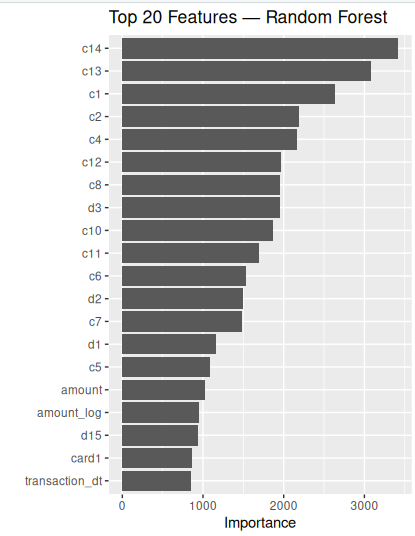
\includegraphics[width=0.78\textwidth]{images/vip_plot.png}
    \caption{Top 20 features ranked by mean decrease in Gini impurity (Random
    Forest). The \texttt{c}-series Vesta count features dominate. Transaction
    amount appears only at rank 16.}
    \label{fig:vip}
\end{figure}

The dominance of \texttt{c14} and \texttt{c13} over raw transaction amount tells a
clear story: fraud in this dataset is driven by \textit{behavioural patterns} ---
unusual transaction counts and timing --- rather than transaction size alone.
The \texttt{d}-series time-delta features also score highly, confirming that timing
is meaningful. A fraudster making small, repeated transactions across a short window
is far more suspicious than a single large purchase.

% ============================================================
\section{Shiny Dashboard}
% ============================================================

The Shiny dashboard serves as the human interface to the model's outputs, reading
live from the \texttt{models.predictions} PostgreSQL table at runtime.

\begin{figure}[H]
    \centering
    \begin{subfigure}[b]{0.48\textwidth}
        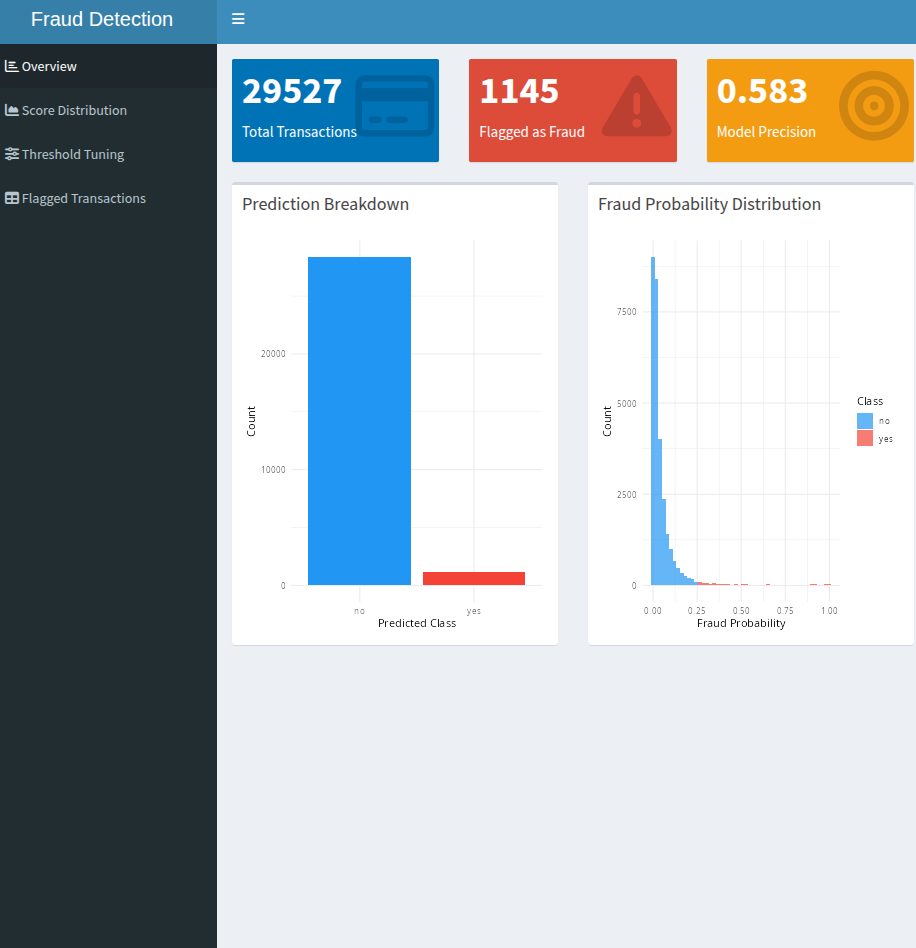
\includegraphics[width=\textwidth]{images/dashboard_overview.png}
        \caption{Overview: KPI summary boxes and prediction breakdown}
    \end{subfigure}
    \hfill
    \begin{subfigure}[b]{0.48\textwidth}
        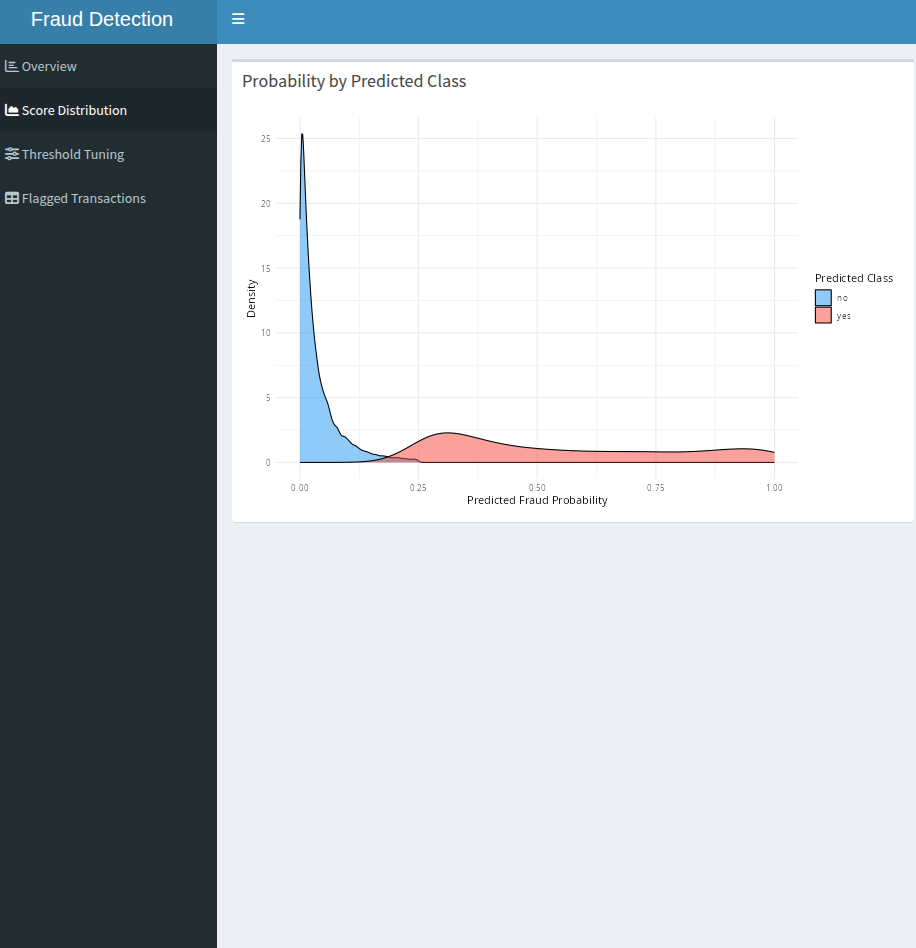
\includegraphics[width=\textwidth]{images/dashboard_scores.png}
        \caption{Score Distribution: density curves by predicted class}
    \end{subfigure}
    \vspace{0.5em}
    \begin{subfigure}[b]{0.48\textwidth}
        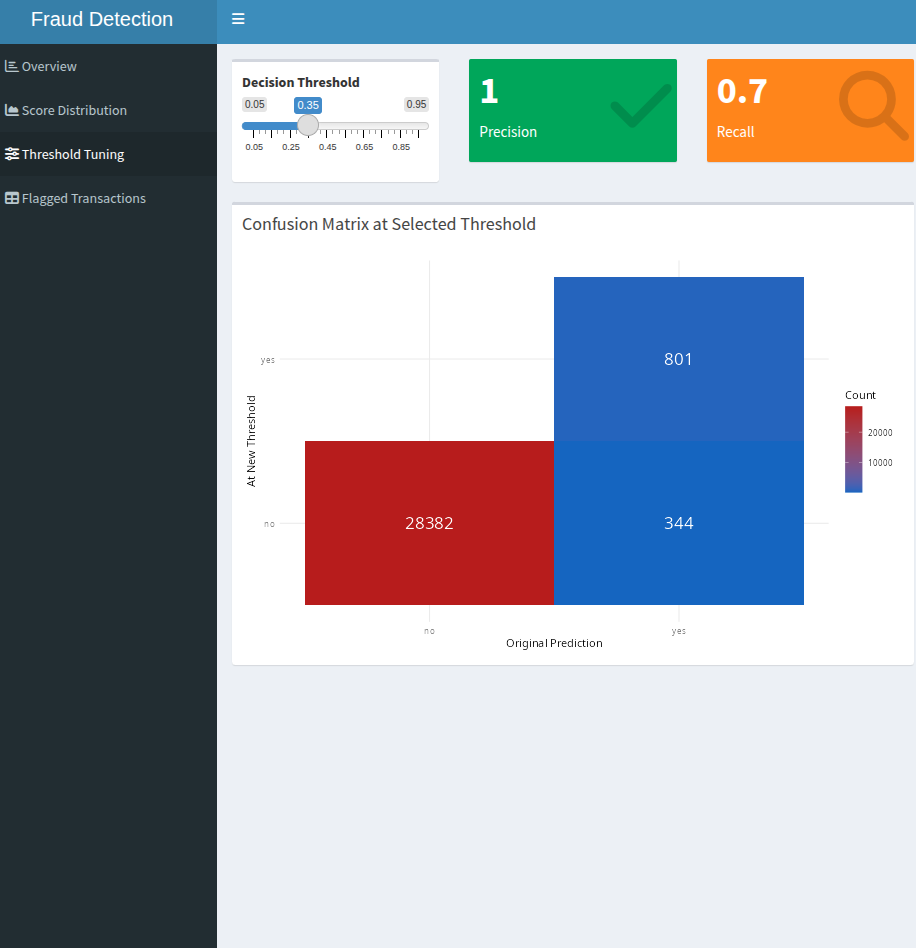
\includegraphics[width=\textwidth]{images/dashboard_threshold.png}
        \caption{Threshold Tuning: live precision and recall at any $\tau$}
    \end{subfigure}
    \hfill
    \begin{subfigure}[b]{0.48\textwidth}
        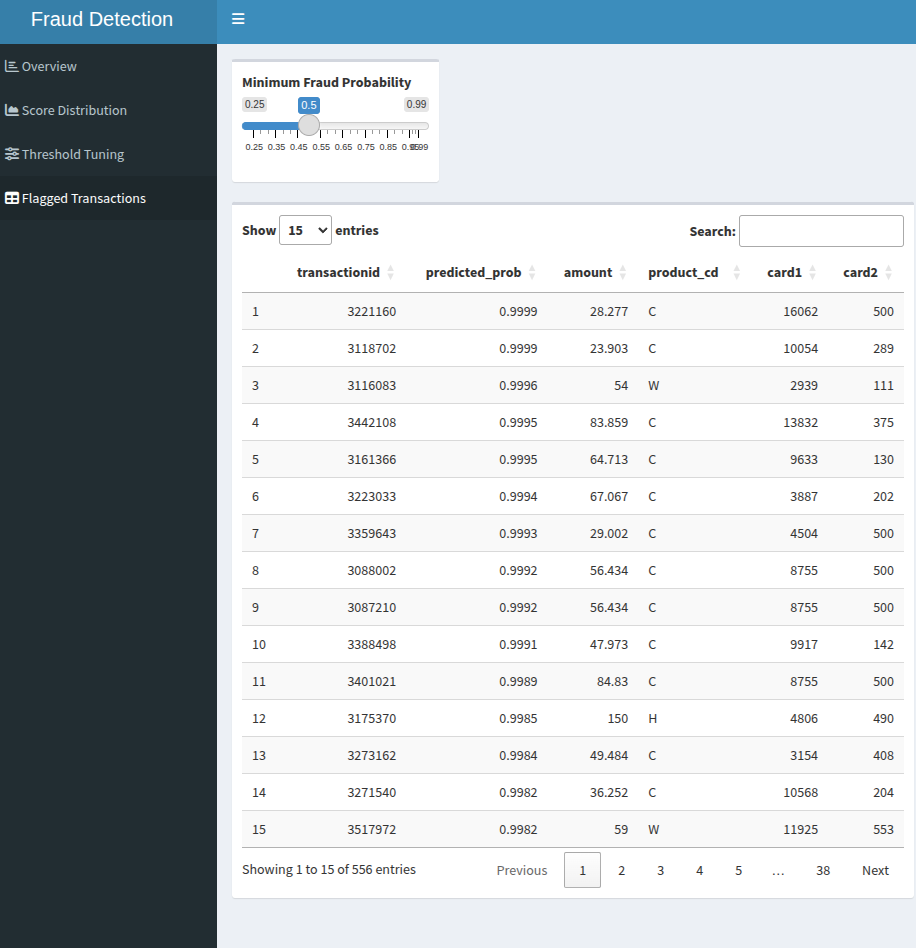
\includegraphics[width=\textwidth]{images/dashboard_table.png}
        \caption{Flagged Transactions: sortable table above a set minimum score}
    \end{subfigure}
    \caption{All four tabs of the Fraud Detection Shiny dashboard.}
    \label{fig:dashboard}
\end{figure}

\textbf{Tab 1 (Overview)} shows 29,527 total test transactions with 1,145 flagged
at the default threshold, alongside prediction breakdown and fraud probability
distribution charts. \textbf{Tab 2 (Score Distribution)} shows overlapping density
curves illustrating the degree of separation between fraud and legitimate transaction
scores --- a useful visual check of model quality. \textbf{Tab 3 (Threshold Tuning)}
is operationally the most useful: a fraud analyst can move the slider and instantly
see precision, recall, and a live confusion matrix update in response. \textbf{Tab 4
(Flagged Transactions)} lists every transaction above a set minimum fraud probability,
sorted by score. Note that transactions 3221160 and 3118702 both score 0.9999 ---
the model is essentially certain they are fraud.

% ============================================================
\section{Future Work}
% ============================================================

The following extensions are planned as hardware and time allow:

\begin{enumerate}
    \item \textbf{Full dataset training} on a cloud instance with sufficient RAM,
    removing the 25\% sampling constraint applied throughout this project.
    \item \textbf{Cross-validated hyperparameter tuning} using \texttt{tune\_grid()}
    with a racing strategy via the \texttt{finetune} package.
    \item \textbf{Model stacking}: combine Random Forest and XGBoost probability
    scores through a meta-learner, which consistently outperforms individual models
    on this dataset class \cite{leborgne2022}.
    \item \textbf{Graph-based features}: construct a card-email-device transaction
    network and compute per-node PageRank and community fraud rates, a key ingredient
    in top Kaggle solutions for this dataset.
    \item \textbf{Concept drift monitoring}: integrate a Population Stability Index
    (PSI) check on incoming score distributions to trigger retraining when the fraud
    distribution shifts.
    \item \textbf{Dashboard deployment} on \texttt{shinyapps.io} for persistent
    public access and portfolio demonstration.
\end{enumerate}

% ============================================================
\section{Conclusion}
% ============================================================

This project built a complete, reproducible fraud detection pipeline using only
open-source tools on a Ryzen 5 laptop with 16 GB of RAM. That constraint is not a
footnote --- it is part of the contribution. Access to meaningful data science
should not require cloud budgets or institutional infrastructure.

The Random Forest classifier achieves a PR-AUC of 0.679 and captures 66.3\% of
fraud cases at 58.3\% precision after threshold tuning at $\tau = 0.25$. The
architecture --- data flowing through four PostgreSQL schemas into a
\texttt{tidymodels} pipeline and out to a live Shiny dashboard --- mirrors
production deployment patterns used in financial services. The limitations are
documented honestly, the code is on GitHub, and the next steps are clear.

Game on.

\newpage
\bibliographystyle{plain}
\begin{thebibliography}{99}

\bibitem{acfe2022}
Association of Certified Fraud Examiners (2022).
\textit{Report to the Nations: 2022 Global Study on Occupational Fraud and Abuse}.
ACFE, Austin, TX.

\bibitem{breiman2001}
Breiman, L. (2001).
Random forests.
\textit{Machine Learning}, 45(1):5--32.

\bibitem{chawla2002}
Chawla, N.V., Bowyer, K.W., Hall, L.O., and Kegelmeyer, W.P. (2002).
SMOTE: Synthetic minority over-sampling technique.
\textit{Journal of Artificial Intelligence Research}, 16:321--357.

\bibitem{chen2016}
Chen, T. and Guestrin, C. (2016).
XGBoost: A scalable tree boosting system.
In \textit{Proceedings of the 22nd ACM SIGKDD International Conference on
Knowledge Discovery and Data Mining}, pages 785--794.

\bibitem{gama2014}
Gama, J., \v{Z}liobait\.{e}, I., Bifet, A., Pechenizkiy, M., and Bouchachia, A.
(2014).
A survey on concept drift adaptation.
\textit{ACM Computing Surveys}, 46(4):1--37.

\bibitem{ieee2019kaggle}
IEEE Computational Intelligence Society (2019).
IEEE-CIS Fraud Detection.
Kaggle Competition Dataset.
\url{https://www.kaggle.com/c/ieee-fraud-detection}

\bibitem{kimball2013}
Kimball, R. and Ross, M. (2013).
\textit{The Data Warehouse Toolkit: The Definitive Guide to Dimensional Modeling},
3rd edition. Wiley.

\bibitem{kuhn2022}
Kuhn, M. and Wickham, H. (2022).
\textit{Tidy Modeling with R}. O'Reilly Media.
\url{https://www.tmwr.org}

\bibitem{leborgne2022}
Le Borgne, Y.A., Siblini, W., Lebichot, B., and Bontempi, G. (2022).
\textit{Reproducible Machine Learning for Credit Card Fraud Detection ---
Practical Handbook}.
Universit\'{e} Libre de Bruxelles.

\bibitem{saito2015}
Saito, T. and Rehmsmeier, M. (2015).
The precision-recall plot is more informative than the ROC plot when evaluating
binary classifiers on imbalanced datasets.
\textit{PLOS ONE}, 10(3):e0118432.

\bibitem{vanVlasselaer2015}
Van Vlasselaer, V., Bravo, C., Caelen, O., Eliassi-Rad, T., Akoglu, L.,
Snoeck, M., and Baesens, B. (2015).
APATE: A novel approach for automated credit card transaction fraud detection
using network-based extensions.
\textit{Decision Support Systems}, 75:38--48.

\end{thebibliography}

\end{document}
